\chapter{ニュース番組音声における非発話区間の調査}
本章では、ニュース番組音声の発話間隔の調査を行う。これは、同一話者が連続で発話する場合は次の発話までの間隔が非常に短いと考え、話者が切り替わる際は映像の切り替わりなどがあるため発話の間隔が長いと考えたためである。\par

\section{使用する音声データ}
パラメータの学習用にニュース番組の音声データ13個を用いる。各音声データには、事前に人手で4種類(音楽、音声、雑音、無音)の音源ラベルが付与されている。「音声」の音源ラベルが付与された区間においては、更に発話者の情報が付与されている。また「音声」の音源ラベルをもとに対象の音声データから発話区間を抽出し、それを一発話とした。\par
表\ref{table:train_detail}に検証に用いるデータの詳細を示す。\vspace{0.2in}

\begin{table}[htb]
  \begin{center}
  \label{table:train_detail}
    \caption{パラメータの学習用音声データの詳細}
    \begin{tabular}{|c||c|c|c|} \hline
      データID & 収録時間 & 話者数 & 全発話数 \\ \hline
      ニュースA & 30分3秒 & 20 & 337 \\ \hline
      ニュースB & 30分3秒 & 31 & 312\\ \hline
      ニュースC & 30分3秒 & 21 & 324 \\ \hline
      ニュースD & 30分4秒 & 20 & 324\\ \hline
      ニュースE & 20分3秒 & 13 & 159\\ \hline
      ニュースF & 30分3秒 & 22 & 343\\ \hline
      ニュースG & 30分4秒 & 22 & 313\\ \hline
      ニュースH & 30分4秒 & 20 & 315\\ \hline
      ニュースI & 30分4秒 & 17 & 321\\ \hline
      ニュースJ & 30分4秒 & 16 & 337\\ \hline
      ニュースK & 30分4秒 & 20 & 363\\ \hline
      ニュースL & 30分4秒 & 26 & 345\\ \hline
      ニュースM & 30分4秒 & 26 & 314\\ \hline
    \end{tabular}
  \end{center}
\end{table}
\section{調査結果}
調査結果を図\ref{fig:same_sp}、図\ref{fig:different_sp}に示す。

\begin{figure}[htb]
  \begin{center}
    \includegraphics{./figure/same_sp.eps}
  \end{center}
  \caption{同一話者間の非発話区間の時間情報 \label{fig:same_sp}}
\end{figure}

\begin{figure}[htb]
  \begin{center}
    \includegraphics{./figure/different_sp.eps}
  \end{center}
  \caption{異なる話者間の非発話区間の時間情報 \label{fig:different_sp}}
\end{figure}

以上の結果より、同一話者の発話は連続して行われるため、非発話区間は非常に短く、話者が切り替わる場合は非発話区間が比較的長くなることがわかる。しかし、話者が切り替わる場合でも非常に非発話区間が短くなる場合がある。これは、

\begin{itemize}
\item 対話者による発話中の相槌
\item 対話中の素早い応答
\item インタビューイの切り替わり
\end{itemize}

があるためである。